\subsection{Byte Substitution Layer}
\label{sec:byte-substitution}

Byte Substitution layer can be viewed as a row of 16 parallel S-Boxes, each with 8 input and output bits. 
Each state byte $A_i$ is replaced, i.e. substituted, by another byte $B_i$.

\begin{figure}[h] % 'h' means place the figure here if possible
    \centering
    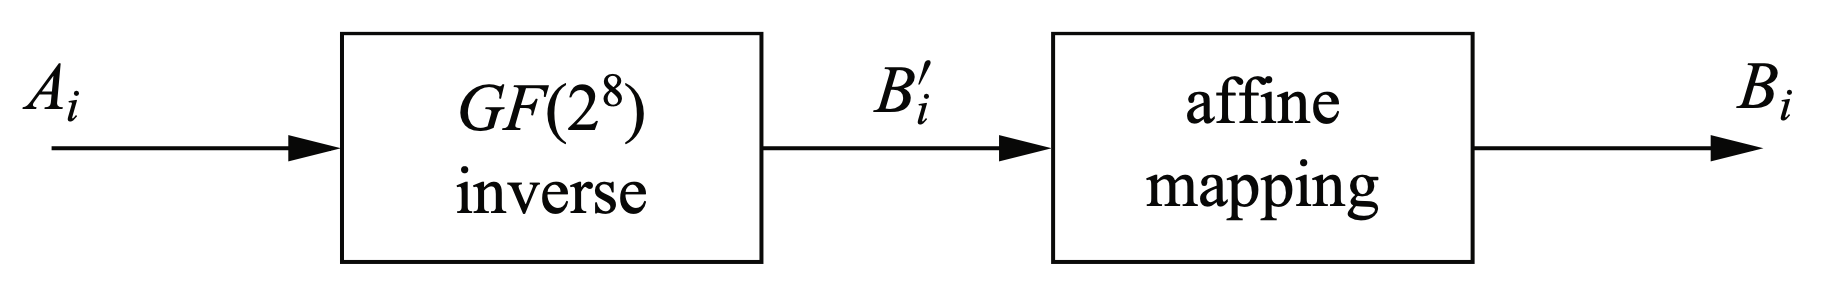
\includegraphics[width=.6\textwidth]{byte-substitution.png} % Adjust width as needed
    \caption{
        The two operations within the AES S-Box which computes the function $B_i = S(A_i)$.
    }
    \label{fig:byte-substitution} % Reference this figure with \ref{fig:sample_image}
\end{figure}

An AES S-Box can be viewed as a two-step mathematical transformation (Figure \ref{fig:byte-substitution}): Galois field inversion and affine mapping.
In software implementations, the S-Box is usually realised as a 256-by-8 bit lookup table with fixed entries.

The advantage of using inversion in $GF(2^8)$ as the core function of the Byte Substitution layer is that it provides a high degree of non-linearty, which provides optimum protection against some of the strongest known analytic attacks. 
The affine step ``destroys'' the algebraic structure of the Galois field, which is needed to prevent attacks that would exploit the finite inversion.

\subsubsection{Galois Field Inversion}

For each input element $A_i$, the inverse ${B'}_i = A_i^{-1}$ is computed (Figure \ref{fig:byte-substitution}).
Both $A_i$ and ${B'}_i$ are considered elements in the field $GF(2^8)$ with the fixed irreducible polynomial $P(x) = x^8 + x^4 + x^3 + x + 1$, such that 
\begin{align}
    A_i \cdot {B'}_i &= 1 \mod P(x)
\end{align}

In AES, the zero element $A_i = 0$ is defined to map to itself, even though the inverse of the zero element does not exist.

\textcolor{red}{Explain with example?}


\subsubsection{Affine Mapping}

Each byte ${B'}_i$ is multiplied by a constant bit-matrix, followed by the addition of a constant 8-bit vector:
\begin{align}
    \begin{pmatrix}
        b_0\\
        b_1\\
        b_2\\
        b_3\\
        b_4\\
        b_5\\
        b_6\\
        b_7
    \end{pmatrix}
    &\equiv
    \begin{pmatrix}
        1 & 0 & 0 & 0 & 1 & 1 & 1 & 1\\
        1 & 1 & 0 & 0 & 0 & 1 & 1 & 1\\
        1 & 1 & 1 & 0 & 0 & 0 & 1 & 1\\
        1 & 1 & 1 & 1 & 0 & 0 & 0 & 1\\
        1 & 1 & 1 & 1 & 1 & 0 & 0 & 0\\
        0 & 1 & 1 & 1 & 1 & 1 & 0 & 0\\
        0 & 0 & 1 & 1 & 1 & 1 & 1 & 0\\
        0 & 0 & 0 & 1 & 1 & 1 & 1 & 1
    \end{pmatrix}
    \begin{pmatrix}
        {b'}_0\\
        {b'}_1\\
        {b'}_2\\
        {b'}_3\\
        {b'}_4\\
        {b'}_5\\
        {b'}_6\\
        {b'}_7
    \end{pmatrix}
    +
    \begin{pmatrix}
        1\\
        1\\
        0\\
        0\\
        0\\
        1\\
        1\\
        0
    \end{pmatrix}
\end{align}
where ${B'} = \left( {b'}_7, \dots, {b'}_0 \right)$

\subsubsection{Lookup Table}

If one computes both steps for all 256 possible input elements of the S-Box and stores the result, one would obtain \textcolor{red}{lookup table}.

\textcolor{red}{Explain with example?}